\documentclass{standalone}
\usepackage{tikz}
\usetikzlibrary{shapes,arrows,positioning,calc,backgrounds,fit}

\begin{document}

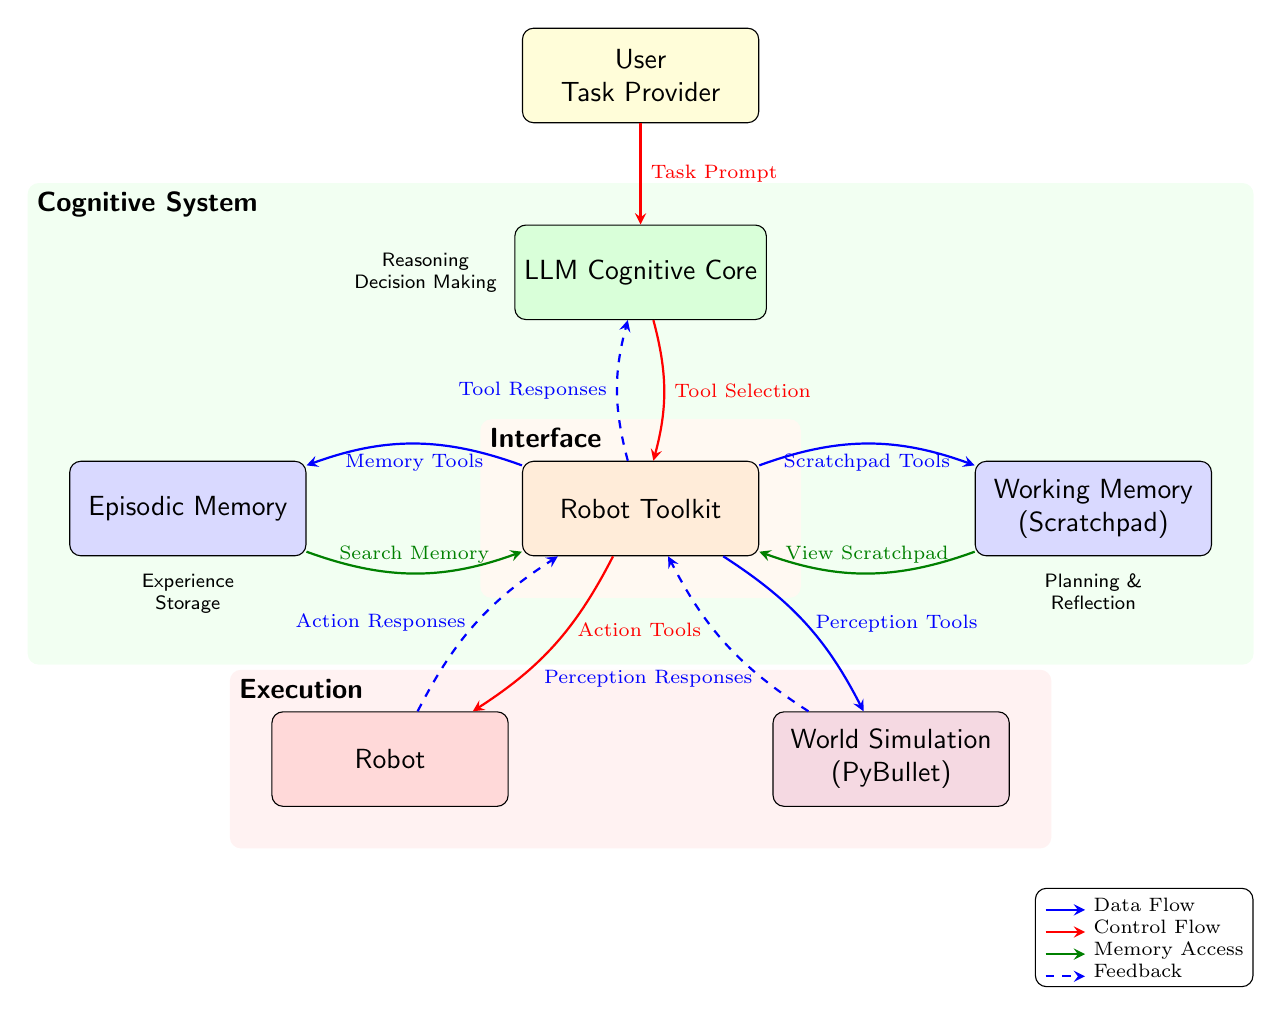
\begin{tikzpicture}[
    node distance=1.5cm and 2cm,
    box/.style={draw, rounded corners, minimum width=3cm, minimum height=1.2cm, align=center, font=\sffamily},
    layer/.style={box, fill=black!10, minimum width=4cm},
    component/.style={box, fill=white},
    memory/.style={component, fill=blue!15},
    cognitive/.style={component, fill=green!15},
    interface/.style={component, fill=orange!15},
    execution/.style={component, fill=red!15},
    simulation/.style={component, fill=purple!15},
    arrow/.style={->, >=stealth, thick},
    bentarrow/.style={arrow, bend left=15},
    dataflow/.style={bentarrow, blue},
    controlflow/.style={bentarrow, red},
    memoryflow/.style={bentarrow, green!50!black},
    label/.style={font=\sffamily\bfseries, align=center}
]


% User node (external to system layers)
\node[component, fill=yellow!15] (user) at (0,9) {User\\Task Provider};

% Cognitive Layer Components
\node[cognitive, below of=user, node distance=2.5cm] (llm) {LLM Cognitive Core};

% Technically not part of the cognitive layer, but needs to be defined here
\node[interface, below of=llm, node distance=3cm] (toolkit) {Robot Toolkit};

% Memory compontents
\node[memory, left of=toolkit, node distance=5.75cm] (memory) {Episodic Memory};
\node[memory, right of=toolkit, node distance=5.75cm] (scratchpad) {Working Memory\\(Scratchpad)};

% Interface Layer Components

% Execution Layer Components
\node[execution, below left of=toolkit, node distance=4.5cm] (robot) {Robot};

% Simulation Layer Components
\node[simulation, below right of=toolkit, node distance=4.5cm] (simulation) {World Simulation\\(PyBullet)};

% Connections within Cognitive Layer
\draw[dataflow] (toolkit) to [bend right=20] node[below, font=\scriptsize] {Memory Tools} (memory);
\draw[memoryflow] (memory) to [bend right=20] node[above, font=\scriptsize] {Search Memory} (toolkit);
\draw[dataflow] (toolkit) to [bend left=20] node[below, font=\scriptsize] {Scratchpad Tools} (scratchpad);
\draw[memoryflow] (scratchpad) to [bend left=20] node[above, font=\scriptsize] {View Scratchpad} (toolkit);

% Connection from User to LLM (Task Input)
\draw[controlflow] (user) to [bend left=0] node[right, font=\scriptsize] {Task Prompt} (llm);

% Connections from Cognitive to Interface
\draw[controlflow] (llm) to [bend left=15] node[right, font=\scriptsize, align=left] {Tool Selection} (toolkit);
\draw[dataflow, dashed] (toolkit) to [bend left=15] node[left, font=\scriptsize, pos=0.5] {Tool Responses} (llm);
% \draw[memoryflow] (memory.south) -- ++(0,-0.5) -| node[above right, font=\scriptsize, pos=0.25] {Memory\\Access} (toolkit.north);
% \draw[memoryflow] (scratchpad.south) -- ++(0,-0.5) -| node[above left, font=\scriptsize, pos=0.25] {Reasoning\\Data} (toolkit.north);

% Connections from Interface to Execution
\draw[controlflow] (toolkit) to [bend left=15] node[right, font=\scriptsize, pos=0.4] {Action Tools} (robot);
\draw[dataflow, dashed] (robot) to [bend left=15] node[left, font=\scriptsize, align=right] {Action Responses} (toolkit);

% Connections from Execution to Simulation
% \draw[controlflow] (robot) to [bend left=15] node[above, font=\scriptsize] {Physics\\Interaction} (simulation);

% Feedback connections (simulation -> Execution -> Interface -> Cognitive)

% Perception tools
\draw[dataflow, dashed] (simulation) to [bend left=15] node[left, font=\scriptsize, align=right, pos=0.25] {Perception Responses} (toolkit);
\draw[dataflow] (toolkit) to [bend left=15] node[right, font=\scriptsize, pos=0.5] {Perception Tools} (simulation);

% Tool details (around toolkit)
% \node[below=0.3cm of toolkit, font=\scriptsize\sffamily, align=center] (tools) {
%     \begin{tabular}{c}
%         look\_around() \\
%         move\_to() \\
%         grab() \\
%         place() \\
%         search\_memory() \\
%         end\_task() \\
%         scratchpad\_ops()
%     \end{tabular}
% };

% Annotations
\node[left=0.1cm of llm, font=\scriptsize\sffamily, align=center] (reasoning) {Reasoning\\Decision Making};
\node[below=0.1cm of memory, font=\scriptsize\sffamily, align=center] (experience) {Experience\\Storage};
\node[below=0.1cm of scratchpad, font=\scriptsize\sffamily, align=center] (planning) {Planning \&\\Reflection};

% Define layers with background rectangles that automatically resize
\begin{scope}[on background layer]
    \node[fill=green!5, rounded corners, fit=(llm) (memory) (scratchpad) (reasoning) (experience) (planning), inner sep=15pt] (cognitivelayer) {};
    \node[fill=orange!5, rounded corners, fit=(toolkit), inner sep=15pt] (interfacelayer) {};
    \node[fill=red!5, rounded corners, fit=(robot) (simulation), inner sep=15pt] (executionlayer) {};
    % Explicit layer labels at top left corners
    \node[label, anchor=north west] at (cognitivelayer.north west) {Cognitive System};
    \node[label, anchor=north west] at (interfacelayer.north west) {Interface};
    \node[label, anchor=north west] at (executionlayer.north west) {Execution};
\end{scope}


% Legend
\node[draw, rounded corners, fill=white, align=left, font=\scriptsize, anchor=north east] at ($(current bounding box.south east)+(0,-0.5)$) {
    \tikz\draw[dataflow] (0,0) -- (0.5,0); Data Flow\\
    \tikz\draw[controlflow] (0,0) -- (0.5,0); Control Flow\\
    \tikz\draw[memoryflow] (0,0) -- (0.5,0); Memory Access\\
    \tikz\draw[dashed, dataflow] (0,0) -- (0.5,0); Feedback
};

\end{tikzpicture}

\end{document}